\section{attic}

\subsection{Kinds of Relations}
    
%%\jmh{Ack ... deductive rules are unsafe, and technically Datalog-neg forbids them due to the free variable in the head.  So you will need to expand your language to include an acceptable notion of per-timestep safety (as Maier suggested), at which point it's not a subset of Datalog-neg.  Would be nice to be able to say ``Dedalus is a subset of (Datalog + \{set of addons\})'' but that would require defining the acceptable saftey before defining timestamps (which are a restriction).}
%\nrc{Title is too long: EDB, IDB, and NDB instead?}
In a \lang program, there are three kinds of relations:
extensional, {\em intensional} or {\em nondeterministic}.

%\nrc{We define the term ``extensional predicate'' before, but not
%  ``extensional relation''.}
\begin{definition}
%
An \emph{intensional} relation is a relation that appears
in the head of one or more atemporal or inductive rules in the program, but
never in the head of an asynchronous rule.~\nrc{``atemporal'' rules
  have not been defined.}
%
\end{definition}
\begin{definition}
%
A \emph{nondeterministic} relation is a relation that
appears in the head of one or more asynchronous rules in the program.
%
\end{definition}
We refer to the sets of ground atoms in intensional and nondeterministic
predicates respectively as the IDB, and NDB.

%\jmh{introduction of the MDB doesn't seem useful, actually.  I'd drop this,
%and if you need to define a ``mutable'' relation as one that participates in
%the head of a temporal rule, you can do so as needed.}
The EDB, IDB, and NDB are all pairwise disjoint.  Intuitively, the distinction
between the NDB and IDB is that the NDB is determined nondeterministically~\nrc{clumsy} from
the EDB, IDB and NDB, while the IDB is determined deterministically from the
EDB, IDB and NDB.  Thus, given a \lang instance, all IDB predicates that do
not transitively depend on NDB predicates can be evaluated deterministically.
We will refer to facts, ground atoms in the EDB, and \emph{events}
interchangeably, for reasons which will soon become clear.
%%\jmh{The only reason to worry about the MDB being non-deterministic is @sync, which you didn't in fact need to introduce yet.  Again, I don't see this discussion being useful.}

\subsection{Traces}


\begin{figure}[t]
  \centering
  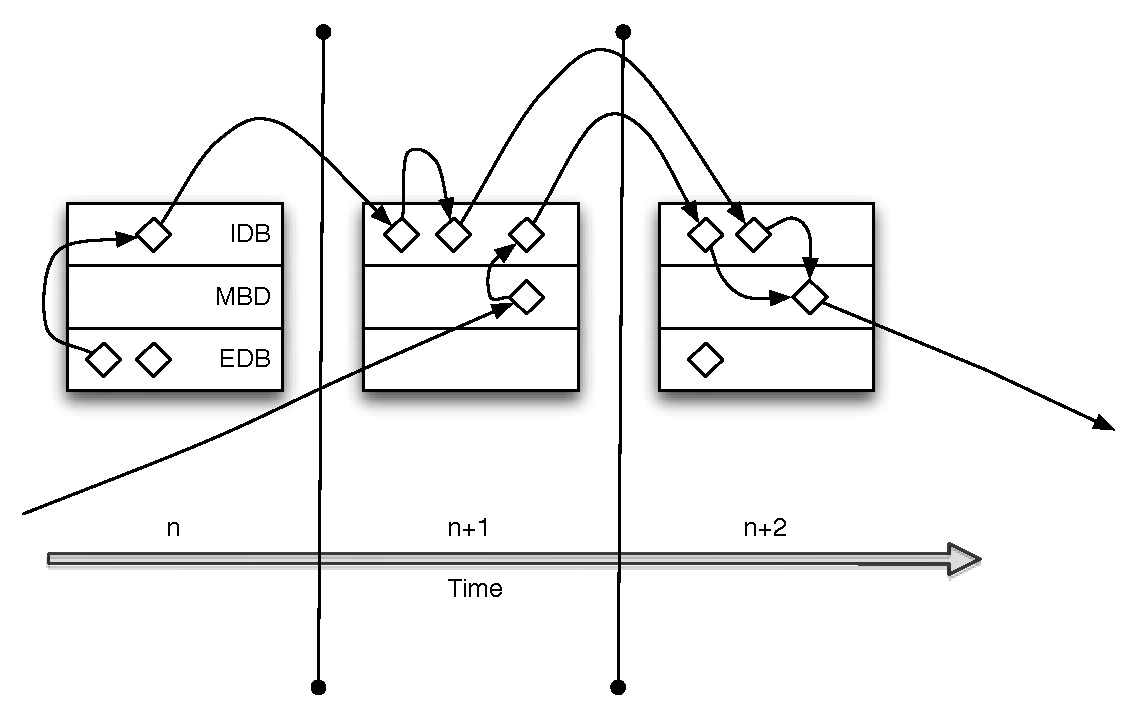
\includegraphics[width=1\linewidth]{edbidbmdb.pdf}
  \label{fig:edbidbmdb}
  \caption{Derivations across time in IDB and MDB relations.}
\vspace{-8pt}
\end{figure}

\paa{this section (its placement \emph{and} content) is somewhat problematic given the current structure
of the draft.  We've established the notion of finite prefixes of a (possibly infinite) EDB.  A trace is basically just
an interpretation (a set of ground atoms) -- by calling it a ``trace" we're connoting a post-hoc interpretation.
A trace that is just EDB is sufficient, given a program, to augment the trace with IDB and MDB atoms such that
the resulting trace is a model (by simply running a fixpoint computation).  For a program with no async rules, the EDB of input is sufficient to recreate the
program execution exactly -- that is to say, to reproduce the single minimal model of the program given the EDB.
It is \emph{not} sufficient to recreate the execution of a program with async rules: intuitively, we'd need to include in 
the trace the complete MDB, for every entry in it potentially corresponds to one of many possible minimal models.
perhaps we just want to show that there is a method (drop the async rules and run a fixpoint computation to generate
the IDB from MDB and EDB) to regenerate a "complete trace" (ie minimal model) from EDB $\cup$ MDB}

%Consider a non-empty EDB $E$, an empty MBD $M$ and IDB $I$ and a program $P$.  Evaluating $P$ against $E$ may derive facts in $M$ and $I$.

\begin{definition}
A \emph{trace} is any set of facts from the EDB, MDB or IDB of a Dedalus program evaluation.
\end{definition}

Any trace for a Dedalus instance $(P,E)$ is an interpretation of $(P,E)$.
%\wrm{lol, why do we need the notion of an incomplete trace?}

\begin{definition}
%
A \emph{complete trace} of an evaluation of a Dedalus instance is the union of
the given EDB with the derived IDB and MDB.
%
\end{definition}

\begin{lemma}
%
A complete trace of a Dedalus instance $(P,E)$ is its unique minimal model.
%
\end{lemma}

%\begin{lemma}
%%
%For any bound on $successor$, a complete trace of a Dedalus instance $(P,E)$ has a unique minimal model.
%%
%\end{lemma}

If we evaluate E given P, and P is stratifiable, the resulting set of ground atoms is a minimal model.
In our case, however, successor causes our EDB to be infinite, so the minimal model of any Dedalus program 
with temporal rules is potentially infinite.  \paa{but we'd like to show that a weaker property holds: that for any value $N$
in the \emph{successor} relation, the resulting program has a minimal model.}
\wrm{we either already showed this, or our theorems above are wrong.}


\begin{definition}
A \emph{minimal trace} is a subset of a complete trace that excludes any IDB ground atoms derived through an inductive
rule.
\end{definition}

A minimal trace of a Dedalus program $P$ is equivalent to the complete trace of which is is a subset -- the latter may be derived from the former by repeated
applications of inductive rules.  However, a given a Dedalus instance $(P, E)$ and a minimal trace T (where $E \subset T$), a fixpoint
computation will most likely \emph{not} yield a minimal model, because new tuples may be added to the MDB that represent a component 
of a different minimal model, and because these may affect the IDB.  The set of ground atoms $EDB \cup MDB_{old} \cup IDB_{new}$
\emph{may} may be a minimal model, iff $IDB_{new} = IDB_{old}$.  \paa{actually I am not sure if that is true}.  
$(EDB \cup MDB_{old} \cup IDB_{new} \cup IDB_{old})$ is certain to be a model, but is only minimal if $IDB_{new} \subset IDB_{old}$.

A minimal trace records the nondeterminism caused by the delay or reordering of async rules, and
is equivalent to the original program execution.  

\begin{definition}
A \emph{reduced trace} is a minimal trace with normalized time suffixes starting with 0 and increasing by 1 at each step.
\end{definition}

show a (trivial) procedure for reduction and make some claims about equivalences without entanglement.

\begin{definition}
A \emph{event trace} is a Dedalus EDB.
\end{definition}

An event trace and program P may be used to generate a new IDB and MDB.  The MDB is virtually certain to differ from that of another
execution, while the IDB may differ, depending on its dependency on the MDB.  The union of these three databases is of course a
minimal model, but probably not the same minimal model from another execution.  \paa{but can we say that it will often be true that if we project 
out the time attribute from every predicate, the minimal models will be the same? it won't always be true...}





